% 
% PhD Project Protocol
% Maxime Lavigne
%
\documentclass[12pt]{memoir}
\usepackage[utf8x]{inputenc}
\usepackage[letterpaper, margin=2cm]{geometry}
\usepackage{hyperref}
\usepackage{lipsum}
\usepackage{graphicx}
\usepackage{atbegshi}
\usepackage[toc,section=chapter]{glossaries}
\usepackage{wrapfig}
\usepackage{todonotes}
\usepackage[final]{pdfpages}

\makeglossary

% Default, Single Space equals 6 lines per inch exactly.
\chapterstyle{bringhurst} % -- the real good one
%bringhurst
%culver
%komalike
%\chapterstyle{komalike}

\renewcommand{\clearforchapter}{}

\renewcommand{\section}[1]{%
  \refstepcounter{section}%
  \addcontentsline{toc}{section}{\thesection \quad #1}%
  \vspace{0.25cm}
  \textbf{\large\thesection.}%
  \space\nolinebreak \large\textbf{#1}\normalsize \quad}

% Disable hskip warning during table of content generation
\pdfstringdefDisableCommands{%
  \let\enspace\empty  % this causes the warning for \kern
  \let\noindent\empty % this causes the warning for \indent
  \let\hskip\empty
}
\newglossaryentry{AF} { name=A\&F, description={ Audit and Feedback } }
\newglossaryentry{CRF} { name=CRF, description={Case Report Form} }
\newglossaryentry{DW} { name=DW, description={Data warehouse} }
\newglossaryentry{EAF} { name=e-A\&F, description={Electronic Audit and Feedback} }
\newglossaryentry{HF} { name=HF, description={Heart Failure} }
\newglossaryentry{ICU} { name=ICU, description={Intensive Care Unit} }
\newglossaryentry{QI} { name=QI, description={Quality Improvement} }
\newglossaryentry{MUHC} { name=MUHC, description={McGill University Health Centre} }
\newglossaryentry{RCT} { name=RCT, description={randomized control trial} }


\begin{document}

\pagestyle{plain}

\AtBeginShipoutNext{\AtBeginShipoutNext{\AtBeginShipoutDiscard}}
\begin{titlingpage}

\begin{minipage}[c]{0.23\textwidth}
\raggedright 

\includegraphics[width=0.75\linewidth]{coa.jpg}
\end{minipage}%
\vrule width 2pt
\begin{minipage}[c]{0.73\textwidth}
	\centering
	
	\vspace{5cm}
	{\huge\scshape Improving your\\Clinical Practice \\ \vspace{0.5cm} for the Game's Own Sake}
	
	\vspace{2cm}
	{\Large\bfseries Thesis Protocol\par}
	
	\vspace{2cm}
	{\Large\itshape Maxime Lavigne\par}
	
	\vspace{2cm}
	supervised by\par
	Dr.~David L. \textsc{Buckeridge}
	
	\vspace{2cm}
	thesis committee\par
	Dr.~Noah \textsc{IVERS}\par
	Dr.~Robyn \textsc{TAMBLYN}\par

	\vspace{2cm}
	{\large Nov 15, 2019\par}
\end{minipage}%

\end{titlingpage}

\tableofcontents
\thispagestyle{empty}
\clearpage

% Pages Plan
% Intro 3/4
% Goal  1/4        p1
% Back  1          p2
% Common Meth. 1/2
% Data Source 1    p3 p4.5
% Objective 1 1.5  p4.5 p6
% Objective 2 1.5  p6 p7.5
% Objective 3 2    p7.5 p9.5
% Limitations .5   p10
% Contribution 3/4 
% Conclusion 1/4   p11

\setcounter{page}{1} 
\chapter{Introduction}
Audit and feedback (\gls{AF}) is an increasingly used quality improvement technique defined as a summary of the clinical performance of healthcare providers over a specified period of time. In essence, A\&F assesses providers' performance and compares it with established standards to then provide a summary designed to drive improvement.\cite{ivers2012audit}

There are multiple reasons why some institutions choose to use A\&F. For example, it is known that unintended and inappropriate variation in care are common, and that clinicians are relatively poor at self-assessment.\cite{davis2006accuracy} Additionally, A\&F is known to be a scalable and relatively inexpensive strategy to promote the uptake of best practices found in high-performing health systems.\cite{baker2015creating}. The added attention A\&F receives is encouraging as its improvements, even if small, could result in clinically meaningful and cost effective changes in processes and outcomes.\cite{ivers2018using}

Yet, designing effective A\&F remains difficult. The latest Cochrane reiterated that "[A\&F] will continue to be an unreliable approach to quality improvement until we learn how and when it works best."\cite{foy2005we} This is why the literature explores myriad aspects of its implementation, how it measures care, how it communicates its findings, and through what mechanisms it operates. As theories of decision making suggest, one particularly appealing lever are the  incentives surrounding certain practices. Research on incentives in A\&F has largely been targeted at the use of extrinsic motivators be it monetary\cite{campbell2007payperf}, social\cite{ehrenfeld2014automated}, or reputational\cite{schneider1998use}. This research led to encouraging results but also presented limitations. As an example, a review of pay-for-performance showed potential short term improvement in the process of care but little to no effect effect on intermediate health outcomes.\cite{mendelson2017effects} Authors pointed out some extrinsic rewards have consistent detrimental effects on intrinsic motivations and therefore on important motivators such as accomplishment, mastery and/or self-fulfillment\cite{deci1999meta}. Often characterised as playing the game for the game's own sake.

Behavioural techniques promoting intrinsic motivators exist but their effect on A\&F are unknown. Prior exploration of effective goal setting theory and self-determination theory suggest it could have a clear and beneficial impact on A\&F. Especially through the use of interactive and low-latency summaries such as those used in electronic A\&F. Gamification was shown to positively impact two important factors of an ongoing feedback system; engagement and enjoyment.\cite{hamari2014does}

\vspace{0.5cm}
\chapter{Research Objectives}
My research goal is to study the effect of gamification, a behavioural intervention, on electronic audit and feedback (\gls{EAF}).  My hypothesis is that gamification will increase the adoption, retention, and engagement with \gls{EAF}, in comparison to a traditionally designed system. This hypothesis addresses important gaps in evidence regarding the application of gamification and related behavioral theories to \gls{EAF}. I propose a manuscript-based thesis with three objectives:

\begin{enumerate}
    \item Develop a set of quality indicators for \gls{EAF} to assess and improve the appropriateness of heart failure management at the MUHC.
    \item Assess the usability and usefulness of gamified \gls{EAF} for physicians at the MUHC.
    \item Estimate the effect of gamification on the adoption, engagement, and effectiveness of e-A\&F at the MUHC.
\end{enumerate}

% "Generally accepted way", will I measure this?
%   - Yes and no.
%     > yes, in the sense that more acceptance means more adoption and engagement
%     > yes-ish, in the sense that this will be touched on in usability metrics
%     > no, in the sense a proper assessment of it would require a qualitative analysis.

% 1 - Are you sure you want to talk about "effect" instead of "association"
%   - There are some limitation to my study, but I'm still doing an RCT. If this is one of the
%     best design to infer causality based on the counterfactual model.
% 2 - Footnote about what traditional system is? It's juste what is done currently

\clearpage
\chapter{Background}
\section{Audit and Feedback}
Audit and Feedback (\gls{AF}) is widely described as a “summary of the clinical performance of healthcare provider(s) over a specified period of time”\cite{ivers2012audit}. Although inclusive, the broad nature of this definition gives the deceptive impression that A\&F is simple to implement. Taken together with evidence on  A\&F potential effects on health professional behaviour and patient health, it could be misunderstood as saying that any summary of performance will improve practice. Yet, as the latest Cochrane review concluded, it is not the case.\cite{ivers2012audit}.

Recent research has focused on theoretical grounding for A\&F \cite{hysong2017theory}\cite{brown2019clinical}\cite{landis2015computer}, identifying characteristics of successful interventions \cite{ivers2012audit}\cite{colquhoun2013systematic}\cite{tuti2017systematic}, and developing evidence-based strategies for adapting and refining A\&F systems \cite{brehaut2016practice}\cite{mcnamara2016confidential}. Through this research, the field moved towards finding better ways of designing effective interventions and predictably discovered many overlaps with the theories and mechanisms of behaviour change\cite{colquhoun2017advancing}.

% While the evidence is evolving, it is unclear how this evidence is being translated into everyday practice. With the increased availability of routinely collected clinical data for the purpose of quality improvements, A\&F interventions are often created in an ad hoc manner. This situation could represent a significant lost opportunity in terms of potential clinical improvements, scientific advances, and better health outcomes.

\section{Motivation and Gamification}
Motivation is a core concept of goal-directed activities along with goal commitment, goal importance, self-efficacy, task complexity, and the availability of feedback. There are two types of motivations; intrinsic (or internal) and extrinsic (or external) motivation. Both influence the satisfaction one gets from accomplishing their goal which then affects their willingness to commit to new challenges and future goals. \cite{locke2002building}

Changing practice is largely about motivating change and consequently there is active research in both the mechanisms that motivate behaviour change \cite{michie2011behaviour} and the impact of A\&F on physicians' intentions\cite{gude2018health}. Prior audit and feedback systems have tried multiple schemes to influence the motivations of health professionals. Yet, although some offered promising results, more research is needed on finding less costly, more easily accepted, or more effective strategies.

Gamification, or “the process of game-thinking and game mechanics to engage users and solve problems” \cite{zichermann2011gamification} could offer A\&F system designers a new way of promoting engagement and providing users with more appealing experiences. One author suggests that “When done well, gamification helps align our interests with the intrinsic motivations of our [users], amplified with the mechanics and rewards that make them come in, bring friends, and keep coming back.” \cite{zichermann2011gamification}. Some elements of gamification such as goals, progression, and scores can already be found in health interventions. However, gamification is not about creating games, but merely leveraging game elements.\cite{deterding2011game}

Good game design principles align with theories of behaviour change. For example, the need for goals that grow with the users, or progression, is analogous to the usefulness of proximal goals in goal setting theory \cite{locke2002building}. The importance of exploration relates to the need for autonomy described in self-determination theory. Finally, game design that fosters a sense of ownership and consequence implicitly favours the creation of personal goals instead of assigned goals, another element of effective goal setting \cite{locke1990theory}. Gamification has been shown in online programs to make users spend more time, contribute more, and lead to downstream behaviour change \cite{looyestyn2017does}.

\section{MUHC Heart Failure}
As improvement in care makes more patient survive cardiovascular diseases, more are living with heart failure (\gls{HF}). In 2019 more than 700,000 Canadians live with \gls{HF}.\footnote{From the Canadian Chronic Disease Surveillance System, adjusted for the 2019 population} This is a concern for the McGill University Health Center (\gls{MUHC}), a leading center for cardiovascular research in Canada which treats around 600 patients with \gls{HF} per year. The recent opening of a hospital-wide data warehouse along with the center's strong research portfolio in cardiovascular care creates an appealing opportunity.

% End

\chapter{Methods}
In this section, I describe: 1) the data, 2) a plan for each objective, 3) limitations and  mitigation strategies, and 4) anticipated contributions. The logical thread of the objectives is to understand how to adapt a known strategy to a new context, to develop and validate a prototype solution, and to evaluate the effect of this prototype in this new context. These objectives will be met through a descriptive study to identify suitable quality indicators, a usability study to ensure the gamified system is usable and useful, and a randomized trial to evaluate the effect of gamification on \gls{EAF}.

In the following sections, I describe the design of \gls{AF} the intervention, software engineering practices, and the design and conduct of the \gls{RCT}. In terms of the necessary expertise for the proposed research, I am formally trained in software engineering and have access to the McGill Clinical and Health Informatics software development team. My supervisor is Director of the MUHC data warehouse (DW) and my thesis committee includes Dr. Noah Ivers, a leading worldwide expert on \gls{AF}, and Dr. Robyn Tamblyn, an expert in conducting \gls{RCT}s of computer-based interventions in clinical care settings.

\section{Data Source and Characteristics}
% Data Source and Characteristics.
In this section, I describe the MUHC data warehouse (\gls{DW}) and how I plan to connect with it. A data warehouse is an enterprise data aggregation system which facilitates its collection, analysis, and reporting. The MUHC \gls{DW} is a newly created repository of clinical data connected to the hospital information system. It contains data on most process of care at the hospital and can be used for both quality improvement and research project. Data sources that are currently available include ADT, Medecho, Emergency Department, Medical Imaging, and the ICU registry while pharmacy data is scheduled for later integration. All sources are updated daily.

%The McGill University Health Centre Data Warehouse (MUHC DW) began in 2012 with an infrastructure   grant from the Canada Foundation for Innovation (CFI). Now, over 7.5 billion facts are accessible in 380 million rows, and over 6,000 columns, in 381 database tables. These data are linked together and organized for analyses of populations, with over 5.5 million health care episodes as of 2019, and is continually growing.

\begin{table}[h!]
\centering
\begin{tabular}{l|lllll}
\textbf{Year}       & 18   & 17   & 16   & 15   & 14   \\
\textbf{Patients}   & 1827 & 1739 & 1611 & 1535 & 1637 \\
\textbf{Physicians} & 265  & 269  & 266  & 278  & 278 
\end{tabular}
\caption{Counts of HF patients and their physicians, last 5 years, MUHC DW}
\end{table}

At this moment, no clinical data was obtained and I cannot present estimate for any potential clinical measure. However, a data dictionary is available describing the schema of the available data. I have received support from the director of the MUHC warehouse, Dr. David Buckeridge, for this project. A data request will be placed for any adult patient from the emergency department and intensive care unit identified by their ICD codes.\footnote{From "Get with the Guidelines - Heart Failure", from the American Heart Association}
% GWTG https://www.heart.org/idc/groups/heart-public/@wcm/@hcm/@gwtg/documents/downloadable/ucm_495599.pdf
Assigned to each patient, I will request the physician who signed the discharge, and their attending if present. Summary counts are presented in table 4.1. In case where both a resident and an attending are assigned to a patient, both will be considered responsible.

This project will use two datasets coming from the same source. A first, broader and denominalized, data request will be made for the purpose of finding targets in objective one and two. This request will be placed to the research pipeline of the data warehouse. At this point, unique anonymous IDs are sufficient. A second, precise, targeted, and nominalized data request will be made for the purpose of conducting the RCT. During this phase, I need to have the right provider see the right feedback, but these providers also need to see which patient might be in need of additional actions. All data collected by the systems will be linked to anonymous IDs.

All nominalized data will be kept in a remote secure server in the MUHC network. Feedback will also be created by the systems on this server. Anonymous data will be kept on a secure password protected computer, where the data analysis will also take place. All nominalized data will be removed as soon as the trial is over, while summary description of the anonymous data will be published along with the relevant research articles.

% Unsure about where to put in some graphical representation of the data I have here. Since the DW doesn,t have a good and nice visualization already built.

%\begin{wrapfigure}{r}{10cm}
  %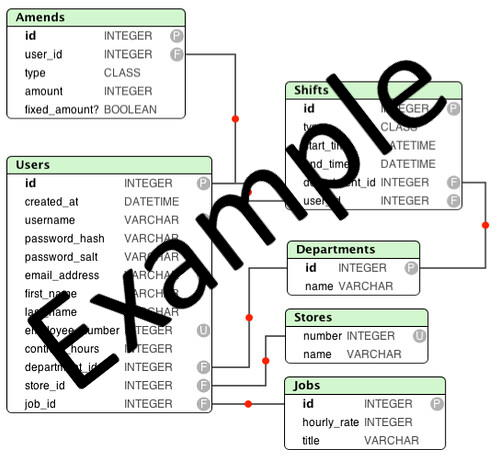
\includegraphics[width=\linewidth]{img/example_erd1.jpg}
  %\caption{Entities and their relationship in the data}
  %\label{fig:entity-relationship-diagram}
%\end{wrapfigure}

%\clearpage
\chapter{Objective 1: Exploration of Metrics}
% Develop a set of quality indicators for e-A&F
% Objective 1 is to develop a set of quality indicators.

% Q1. How many do you need.
% Q2. How do you assess them
% Q3. How do you make a decision after assessing them.

At the core of the ability of audit and feedback to generate insights and induce change is the quality of its measurement. Performance measurement ``seeks to monitor, evaluate, and communicate the extent to which various aspects of the health system meet their key objectives'' \cite{smith2009performance}. A related question then becomes: ``what are the most suitable quality measures for a given care process and a local context?''. The suitability of quality measures will depend on their alignment with an organizational context, their relevance to the actors, their ability to be attributed to specific actors, and their feasibility, accuracy, and reliability \cite{polanczyk2019quality}.

For this first objective, I aim to identify a set of quality indicators for electronic audit and feedback suitable for assessing and improving the appropriateness of heart failure management in adult patients at the MUHC. This set of indicators will be used for both arm of the RCT in objective 3, and its integration is assessed for usability in objective 2.

\section{Research Design}
The study is a single center retrospective exploratory analysis of clinical data from patients with heart failure treated at the McGill University Health Center. Data on the care of adult patients will be obtained for patients discharged from the ED, the ward, or the ICU with heart failure\footnote{From ICD-9 and 10, AHA's, Get with the Guidelines\textsuperscript{\textcopyright} - Heart Failure}. Additionally, I will collect data on the treating physician, the patient's last admission, and any re-admissions to the \gls{MUHC}. For this analysis, one year of data will be collected, as has been done in prior studies of \gls{HF} \gls{AF} \cite{kasje2006educational}. Based on a 5 year average, this approach would include data for 1670 patients discharged by 271 physicians.

There are three aspects to my aim of identifying a set of quality indicators. First, the number of indicators included; second, the criteria for evaluating the indicators; and third, the overall criteria for deciding which indicator to include. For the first question, I am aiming to include approximately 10 indicators, which is similar to the number used in a previous study \cite{matthews2007impact}. There is no clear guidance on the number of indicators in the literature on A\&F, but systems with too few indicators may not contain enough information to engage participants and those with too many may pose a heavy cognitive load resulting in lower usability. For the evaluation of performance indicators, I will use the criteria developed by Campbell (Appendix C for more details)  \cite{campbell2002research} and the characteristics of successful A\&F \cite{ivers2012audit}. Finally, once the attributes of the potential measures are characterised, I will determine the final selection based on a consensus of local substantive experts, my advisors, and myself.

\begin{table}[h!]
\centering
\vspace{-2mm}
\begin{tabular}{c|c}
     \textbf{Campbell's Prerequisites} & \textbf{A\&F Criteria}  \\ 
     \hline
     Acceptability         & Baseline Performance  \\  
     Feasibility           & Availability of Action Plan \\
     Reliability           & Frequency; related to patient load \\
     Sensitivity to change & Latency; time to availability \\
     Predictive value   &  \\
\end{tabular}
\caption{Criteria for the evaluation of quality indicators}
\vspace{-5mm}
\end{table}

\section{Quality Measures}
Multiple efforts have been made between institutions and advocacy groups to define a set of evidence-based, actionable indicators for heart failure \cite{hong2006overview, fonarow2010improving, kelley2006health}. Newer interventions are encouraged to use existing measures instead of developing their own. Doing so accelerates development, contributes to the soundness of the evidence, improves face/content validity, facilitates reproducibility, and promotes the use of measures associated with significant health outcomes \cite{smith2009performance}. 
Candidate measures will be derived from a recent systematic review of quality indicators for the cardiovascular intensive care unit (\gls{ICU}). This list contains 31 \gls{HF} specific and 28 general quality indicators. Example potential indicators include ``length of stay for HF patients'' and ``overall readmission rate'' \cite{goldfarb2018systematic}. Risk adjustment will be performed if needed.

\section{Data and Participants}
Data will be obtained through the MUHC data warehouse. An anonymous ID will be used in place of personal identifiers to minimize the risk of re-identification for patients and care providers in this phase of the research. The data collected for each patient will be drawn from a local adaptation of a recently proposed Lean case report form (\gls{CRF}) for heart failure \cite{psotka2019design}. Validation of a local adaptation of the Lean CRF using data available in the MUHC data warehouse is currently underway. 

Approval from the MUHC research ethics review board will be requested along with a waiver of the need to obtain individual consent from patients and physicians. This dataset and waiver will be reused for objective 2 but not 3. The risk of re-identifying patients and physicians is low due to the use of retrospective, routinely collected anonymized data and the implementation of procedures to store the data securely.

\section{Analysis plan}
The data will be explored using descriptive statistics to represent quality measures along with their completeness and trends over time. Measures will also be stratified by demographic factors, cardiovascular risk, and physician characteristics.

The descriptive statistics will be used to assess the feasibility, presence of valid and reliable data, along with baseline performance possible frequency of update. Stratified analysis will be used to assess the reliability, or how indicators can be reproducibly computed between providers and patients. The same technique is used for sensitivity to change, or the indicator's capacity to detect changes in quality of care. Acceptability is supported by being on the list of candidates, but will also be confirmed by a local expert. Latency will be assessed with DW analysts as the time between an action and presence of data in the system. Availability of an action plan will be checked by going to the original framework of the indicators. Finally, it will be assumed candidate measures have content validity. Predictive value will be assessed only for process indicators, and will be measured as the degree of association between improvement in the indicator and lower HF re-admissions.
% Issues
It could be that no indicators end up being suitable, but it is unlikely given the candidate measures are used in similar healthcare systems. The possibility of incompatibility between the Lean CRF and MUHC data is why I will use a pre-made local adaptation.

% 1 - Exclude stays for patients who died during their stay? Since they can't have readmission.
%   - Would mess with mortality estimates, and it's the same for everyone.
% 2 - The final set will be selected by my advisors and I
%   - What?!? What criteria, how?, how is that replicable.
% 3 - How will you process the predictive validity modeling?
%   - Predictive validity will be measured as the degree of association between the measure and lower HF re-admissions and will only be assessed for HF specific process measures.
% 4 - How to you plan on doing risk adjustment?
%   - APR-DRG, is one solution, by weighted average, something like group 1-2-3
% 5 - Will the quality indicators work for ED, ward, AND ICU were people are much sicker?
%   - I would assume the indicators won't be "irrelevant" for lighter context. From there, the intervention is mainly about getting Health professional to improve their own practice. But social aspects will potentially be adjusted for risk, or stratified against comparable colleagues.


% Acceptability                  - (Somewhat confirmed by being on list, but confirmation by local substantive expert)
% Feasibility                    - (from descriptive statistics)
% Reliability                    - (Stratified analysis by provider to look for irregularities in measures)
% Sensitivity                    - (Stratified analysis by patients and trends in time) See if varies
% Validity                       - (Content Validity assessed by org. framework, degree of association between better measure and lower HF readmission for process measure, for outcome measure assumed predictive) 
% Baseline Performance           - (from descriptive statistics)
% Availability of Action Plan    - (Looking at the framework from which the measures come)
% Frequency                      - (from descriptive statistics)
% Latency                        - (Assesses with DW analyst, as the time from action to system knowing)

% Cut out : Any required risk adjustment will be made based on diagnostic related groups (\gls{APR-DRG}).

%\clearpage
\chapter{Objective 2: Usability testing}
% Lab Usability testing
% Objective 2 : Assess the usability, usefulness, and technical barriers to a gamified \gls{eaf} intervention for physicians at the MUHC.
%
%
The field of \gls{EAF} is emerging and evidence is needed to guide design decisions to maximize usability \cite{brown2016interface}. There is no evidence regarding how design decisions about behavioral factors such as gamification affect the usability of \gls{EAF}. Furthermore, preliminary validation of a gamified system is needed to justify spending the time and resources required for a randomized trial.

Consequently, I aim to assess the usability and usefulness of a gamified \gls{EAF} intervention for physicians at the \gls{MUHC}. A secondary aim will be to identify potential technical difficulties in deploying the system for the \gls{RCT}. This assessment will ensure that the system is usable and is free from obvious defects. The assement  also presents an opportunity to verify that the metrics needed for objective 3 can be automatically collected and to generate pilot data to inform the design of the RCT.

\section{Research Design}
I will perform laboratory-based usability testing of the gamified intervention using a convenience sample of eligible physicians starting with 5 and adding 3 more until saturation is reached. Saturation occurs when adding more participants does not result in additional perspectives \cite{green2018qualitative}. During this evaluation the participants will be asked to accomplish the same set of tasks, using simulated but realistic data. The tasks will test core \gls{EAF} functionalities, using goals from the evaluation of the control system, as well as gamified elements. Usability scores of the gamified system will not be compared to the control, due to their use of a different test methodology and different set of functionalities.

The sample size is influenced by the homogeneity of the users (all physicians with high education), and prior evidence on the relation between sample size and the number of usability problems uncovered \cite{nielsen1993mathematical}. Since the usability of the control was already explored by its authors, only the experimental system will be assessed \cite{brown2016interface}. Usability issues uncovered by this exercise will be used to orient pre-trial software development efforts. This testing is summative, meaning it seeks to examine and evaluate how effectively concepts have been implemented \cite{rubin2008handbook}.

I define usability as ``the extent to which a system, product or service can be used by specified users to achieve specified goals with effectiveness, efficiency and satisfaction in a specified context of use'' \cite{international1998iso} As opposed to usefulness, or the ability of a system to ``provide content that is engaging, relevant, and appropriate to the audience''. Both constructs are often used in user experience design and have strong face and content validity \cite{united2006research}. The secondary aim of identifying technical difficulties will be assessed qualitatively from the experience of the research team in setting up the test. It will serve to adapt the solution, to plan for trial deployment.

\section{Procedure}
Participants will first be required to provide informed consent and then complete a pre-test questionnaire to measure age, gender, specialty, number of year of clinical practice, and familiarity with information technology. Then participants will be presented with a series of tasks to accomplish while ``thinking aloud''. The think aloud procedure provides greater insight into the user's mental model by asking them to verbalize their thoughts. Think aloud sessions can elicit a larger set of usability issues than observation alone \cite{ericsson1980verbal}. A researcher will be present to record the thought process and note any difficulties or confusion as the user performs the tasks. Successful completion will be assessed on a scale of 0 to 4, with 0 meaning the user could only accomplish the task with substantial guidance, and 4 meaning the user solved the tasks without help \cite{rubin2008handbook}. The researcher will only provide guidance if the user seeks help or abandons the task. The provided tasks will be centred on the four main features of \gls{EAF} (described in the next section) along with additional tasks to cover the gamified material. I will create these tasks once the intervention is designed and they will be discussed with my thesis committee.

Upon completing the tasks, participants will be asked to complete a TAM2 (technology acceptance model v2) questionnaire and provide any textual unstructured feedback they might want to share at the same time. The TAM2 questionnaire is a validated instrument for measuring perceived usefulness and perceived ease of use, which are important determinants of the attitudes and intentions related with use behavior \cite{venkatesh2000theoretical}. The TAM2 will collect data on projected adoption, and I will also ask participants to estimate their frequency of use of the inervention in scenarios of low, medium, and high baseline performance and with low and high rates of HF patients.
% More info on TAM2 Based on Theory of Reasoned Action Sub. Cri. : Computer Anxiety, Comp. Playfulness, Comp. Self-Efficacy, external control.

\section{A\&F Systems}
Both the experimental and control versions will use electronic audit and feedback systems following the four key components of \gls{EAF} system interfaces: (1) Summaries of clinical performance; (2) Patient lists; (3) Patient-level data; and (4) Recommended actions \cite{brown2015meta}. The control system will be based on the user experience and interfaces described in the PINGR system \cite{brown2016interface}, but adapted for the measures identified in objective 1 and for the collection of data needed in objective 3. I have contact the creator of PINGR, who has offered to help if I have any questions. The experimental system will be built by the McGill Clinical and Health Informatics (MCHI) software development team. They have many years of experience in system development, in usability testing, and in human centered design \cite{shaban2017pophr, lavigne2013hybrid, buckeridge2016developing}.

The design of the experimental system will be largely driven by 1) the ``GOAL framework'' for gamification in software engineering \cite{garcia2017framework}, and 2) the ``Rules of Play'', which is  the authoritative textbook on game design \cite{salen2004rules}. There are four major category of possible game elements; game dynamics (overarching design), game mechanics (step by step processes), specific components (tangible elements of dynamics and mechanics, and aesthetics (design producing positive affect) \cite{mckeown2016gamification}. In order to maintain alignment with the research aims and user-specific concerns when designing the system, recommendations from gamified interventions in similar settings and with similar users will be followed \cite{mckeown2016gamification}. A scrum based software development methodology will be used for its flexibility with local evolving needs, its use of short fast-paced development phases, and its use of an embedded product owner, which in this case will be a local expert \cite{cohn2010succeeding}. This software development methodology enables the use of an agile model of software development \cite{beck2001manifesto}.

\section{Analysis Plan}
The results of this analysis will be threefold: a per task success score, a thematically organised set of issues and feedback, and a TAM2 based compound usability and usefulness score. Special attention will be taken to elicit possible misunderstandings, or adverse effects. These results will be analyzed to assess the potential influence of demographic factors and how they relate to specific interface elements.

% 1 - The results won't be compared because you used different methodology? Why didn't you use the same then?
% 2 - What if the user fails even after strong guidance.
%   - We assume it's still 0-strong guidance.
% 3 - Does the task scenario need to be validated?
%   - I would say not, other than my committee. 
% => How is mock data generated?
% => Real data will elicit more relevant comment and might be the only way to get participant to dig deeply in what is being presented. However, fake data as the advantage of not being so sensitive. Should we choose individuals that would be participants and show them their own data?
% => Contamination of the usability participants?

% Additional References
% => [Usability Website](https://www.usabilitybok.org/usability-testing)

% Cut out

% \textbf{Technical Feasibility} Will this be hosted in-hospital, would they have access outside the hospital. Mobile or Browser based. If inside the hospital, are there computer there able to connect/view the page. If yes, would they have/be given time to view the page and explore it. +(Use the same network and IT resources, maybe connect to the same kind of portal? To assess if it scales.)
% the size of the eligible  population,

%\clearpage
\chapter{Objective 3: Randomized Evaluation}
% Randomized Control Trial
At this point, I will have identified a set of suitable quality indicators for heart failure at the MUHC and have two \gls{EAF} systems with validated usability and usefulness: a gamified, and a traditional system. I will use these systems to estimate how a behavioural intervention focused on intrinsic motivators (i.e., using the principles of gamification), affects adoption, engagement, and effectiveness of an e-A\&F intervention.

The proposed research design is a single center, parallel-arm, actively controlled randomized control trial (\gls{RCT}) of physicians treating heart failure patients at the \gls{MUHC}. Random assignment will use a 1:1 ratio. Both systems will present feedback based on the quality measures in objective 1. The trial is planned to last 14 months in total. The RCT design was chosen as opposed to an impact evaluation to reduce the bias due to confounding. The intervention will be delivered through a personalized, confidential web-based portal, accessible by navigating to a specific URL on a ward computer or personal device. In this objective, my hypothesis is that there is a difference in adoption of the \gls{EAF} system between the traditionally designed and gamified arms. Similarly, I hypothesize a difference in engagement between the arms. The null hypotheses being that there is no difference in adoption or engagement. I consider effectiveness a secondary objective in this trial as the true effect of the systems might be affected by their adaptation, the length of the trial, or what quality measure our data support.

\begin{figure}[h]
    \vspace{-2mm}
    \centering
    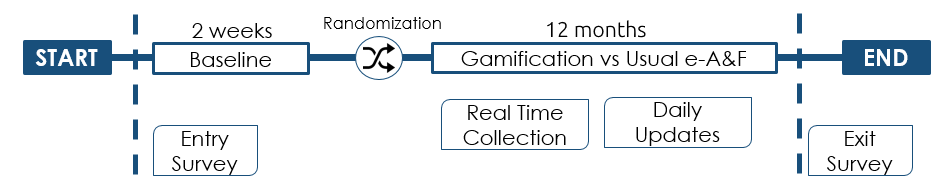
\includegraphics[width=\textwidth]{img/rct_flow_corrected.png}
    \caption{Diagram of the RCT process}
    \label{fig:rct_flow}
    \vspace{-5mm}
\end{figure}

\section{Timing, Participants, and Consent}
To participate in this trial, users must be physicians working at the MUHC, have control over the treatment of patients with heart failure, and work in the emergency department (ED), the ward, or in the intensive care unit (ICU). This population will include attending physicians, medical residents, and fellows. Participants will be followed for a maximum of 12 months after the mandatory 2 weeks baseline assessment. The choice of 12 months was made by balancing feasibility with the need for participants and for enough follow-up to measure retention. No recruitment will be attempted in the last 2 months of the trial. Recruitment will be made by informing the different departments, with recruitment material, and with a local advocate. An email reminder will be sent every 90 days to recommend users to login. Ongoing monitoring will be performed for any signs of harm to patients. Stratified randomization by physician type was considered but dismissed as the likely number of participants (n > 200 for 74\% participation) will make large treatment imbalance unlikely.

% Consent Process
Since only secondary patient data is used, and since it is used as part of the care process, a waiver of patient consent will be requested from the director of professional services. Informed consent will be required from each participating physician and they can stop using either intervention at any time. Participants will not be allowed to switch between arms. If participants inform us of their desire to stop using the interventions, an exit survey will be sent to them.

\section{Data Collection}
No \textit{patient} data will be captured other than to create provider-level feedback. Providers will be able to see nominative data for themselves and their own patients. Both systems will automate indicator processing from patient data as described in the ``data source'' section. Simple randomization will be performed with a 1:1 ratio after a user fills in the entry questionnaire. Both systems will perform real-time data collection as participants use them. Data will be recorded in a secured database, assigned to the anonymous ID of the participant. Participant quality measures will be confidential and will not be shared. All analysis will be performed on participant's anonymous IDs. Participant data will be stored for a duration of 7 years, and any identifier will be destroyed as soon as all data is collected for a participant. Analysts will be blinded to treatment assignment but participants will know from their intervention.

\section{Measures and Outcomes}
Participants will need to complete an entry questionnaire when they first connect to the system. The questions will include basic demographics, same as in objective 2. An exit questionnaire will be sent to participants at the end of the trial. It will be the System Usability Scale (\gls{SUS}), a validated and widely used 10-question tool for measuring perceptions of usability \cite{united2006research}.
% Define and describe how they are collected and at which frequency.
I will use the HEART framework to operationalize the criteria for the third objective. This framework for user-centred metrics addresses previous deficiencies in measuring user experience quality, and providing actionable data. In addition to the primary outcomes (see Table 7.1), secondary outcomes will include: 1) Useless clicks, 2) time on site, 3) number of 90-day periods with at least one non-trivial action \cite{rodden2010measuring}.

\begingroup
\setlength{\tabcolsep}{8pt} % Default value: 6pt
\renewcommand{\arraystretch}{1.5} % Default value: 1
\small
\begin{table}[h!]
\vspace{-2mm}
\begin{tabular}{l|l|l}
\textbf{Measure}       & \textbf{Metric}                  & \textbf{Meaning}                           \\
\hline                                                                                                    
\textbf{Adoption}      & any 2 login, except registration & how many new users start using a product   \\
\textbf{Retention}     & 90-day periods with ≥ 1 login    & how many of the users are still present    \\
\textbf{Engagement}    & logins per 90-day period         & user’s level of involvement with a product \\
\textbf{Effectiveness} & change in quality scores         & success in improving clinical practice
\end{tabular}
\caption{How primary outcomes will be measured}
\vspace{-5mm}
\end{table}
\endgroup

\section{Statistical Plan}
% Descriptive statistics
Descriptive statistics will be used to present the entry survey variables by arm. Categorical data will be summarised by numbers and percentages, and continuous data by mean and standard deviation. Standardized differences will be presented for each variable. Physician flow through the trial will be described using a CONSORT diagram.
% Main Analysis
The results will be analysed using an intent-to-treat approach including all randomized physicians according to the system they where randomized to receive. I do not plan to have interim analysis or a stopping criteria. All applicable statistical tests will be 2-sided and reported at a 5\% significance.

% Main Outcomes
% https://statistics.laerd.com/statistical-guides/independent-t-test-statistical-guide.php
Results for both primary and secondary outcomes will presented along with CI, stratified by arm. In the analysis, I will test the hypotheses that the treatment arm will have: 1) a different proportion of adoption, 2) a different mean retention, and 3) a different mean engagement compared to the control group (see Measures for units). All hypotheses will be tested using a unpaired two-sample t-test. Violations to the assumption of normality will be inspected using a Q-Q plot, and Levene's test for equality of variance will be performed. The t-test is robust to violation of the normality assumption, but if severe variations are found, the Wilcoxon rank sum test will be used. If variances cannot be assumed equal, a Welch-Satterhwaite correction will be applied. For test each, I will report the t-statistic, the degrees of freedom, and the p-value.

% Secondary Outcome
For the secondary outcomes, a composite measure will be created for indicators scaled as percentage representing the average difference in percentage points between the start and end of the trial. Other quality measures will be maintained on their original scale and addressed individually. A similar t-test procedure will be followed, and results will be reported.

% Subgroup analysis
A subgroup analysis of the main outcome will be performed by role (attending or others) and by self-reported familiarity with IT (low, medium, high). Additionally, for exploratory purposes the effect of individual characteristics on adoption, and engagement independent of arm will be modeled using linear regression. Since data can only be missing on the exit survey, and since this survey is only used for explanatory purposes, a complete case analysis will be used. Any feedback of adverse event will be reported. A sensitivity analysis will be performed on the effect of not removing quality indicators. Finally, a t-test of usability score, SUS, will be ran between arms.\footnote{Made following ``Guidelines for the content of statistical analysis plans in clinical trials. \cite{gamble2017guidelines}''}

\section{Sample Size}
To see how many patients and physicians are available, see table \ref{tab:data}. Reporting sample size is complicated by two issues. First, I could not find any baseline data on adoption and retention in \gls{AF}. Second, the population I have is finite and a multi-center study is unfeasible. Hence, this is an estimate for engagement, one of my main outcome. No data was found for \gls{EAF}, so I used a study of gamification in an online education system  \cite{krause2015playful}. The authors hypothesised that gamification could increase retention of users in massively open online courses (MOOC). They reported the mean and confidence intervals for the number of videos viewed, which represents engagement as it marks continuing progress. Since, a more typical rate of engagement for us would be $\approx$ 1 login/90 days, I used scaled engagement measures. The article had 3 groups, testing two aspects of gamification against a control. A sample size calculation (see appendix B) resulted in 177 participants for an effect size of 25\% and 13 for 55\%\footnote{Using the two effect sizes reported in \cite{lachin1981introduction}}, or a participation of 66 and 13\%. A sensitivity analysis was done varying each assumptions to show its effect on power. The calculation was for a two-sided, two-sample t-test with unequal variance, at $\alpha = 0.05$ and $\beta = 0.20$ \cite{lachin1981introduction}.

% Why not :
%
% 0- What if you find *really* different characteristics regardless of randomization, do you adjust?
%
% 1- Crossover
%    Cross-over might not be appropriate due to concerns of carryover effects.
% 2- Stop Rule
%    Difficulty of finding good prior estimate of many measures, and to put a clinically significant
%    threshold on them.
% 3- Why not using a complier average causal effect (CACE) analysis.
%    ???
% 4- How to adjust for people who have diff end - start based on 2 mths vs 12 mths. Less opportunity
%    ??? RCT doesn't care?
% 5- How is power measured in this context?
% 6- How would selection/confounding bias be seen here?
% 7- Does 2 points, end and begin really show a trends.
% 8- Adjustment for multiple testing?
% 9- Adjustement for low Ns confounding?
% 10 - What about recruitement, how to describe or do properly?
% 11 - Add comment about suitability of RCT.
%   - Reduce some type of systematic error (bias).
%   - Especially making participants more exchangeable both from measured and unmeasured factors. (i.e. confounding)
%   - Especially making group similar at baseline.
% 12 - You could say participants will be required to have access to computer but its probably fine.
% 13 - What about contamination and its effect?
%   - Many of the mechanism suggest low effect. (personalized aspect, ownership aspects, and the non-transferable nature of the discrepancy observed) And if it happens, it's likely to dilute the effect.
% 14 - What happens to the data of participants that drop?
%   - As long as they have baseline and 2 90 days period, it's kept.
% 15 - Can I distinguish between what is done by a trainees/mentor or will this always be under the mentor's name?
%    - I assume care is attributable to both the resident and his|er mentor.
%    - Additional details from CB, in the case of trainee, they write the "prescription" for discharge. The prescription is usually counter-signed by the attending. The trainee will also fill-in the summary sheet, which includes the ICD codes, which will be sent to the mailbox of the trainee which will sign it a month later.
% 16 - Could you not use the results from objective 2 in terms of the reported intention to use the system?

% 17 - Is the physician type a confounder of an effect modifier? What is the consequence.
% 18 - What about crossover study?

% Notes
% - The only real way to have exchangeable population based on both measured and unmeasured confounders. Low Ns can nevertheless bring up issues.
% - RCT are especially usefull when the effect is small and bias could therefore mask the effect.
% - Clinical Trials are expensive (Maybe write here about the low cost?)
% - RCT are problematic when outcome is rare. Not the case here.
% - Willcoxon is similar to Mann-Whitney in results.
% Know that 1:1 randomization ratio are the most efficient.


% Cut out 
% Prior research on systems with fewer limits has already shown a positive effect.
% [RCT was chosen to] increase the usefulness of the results it generates by aligning more closely with prior evidence in the field
%  for at least 10 weeks\footnote{Baseline assessment + 2 months}
% Because of the rate and nature our quality measures, a
% each component (effect size, participation rate, and variance) separately

\chapter{Study Limitations}
% Study Limitations and Mitigation
A major challenge in designing this electronic audit and feedback system is, in collaboration with the clinical team, find quality improvements topics which are important for the users, have data and quality standards available, and are appropriate targets for A\&F. This also means having clinical partners which are willing to take time to participate in the governance of this project. These partners are essential when planning an implementation to prevent rejection, lack of trust, or perceived intrusion. Physicians wont be remunerated for their participation, but a request will be made for them to get continuing medical education (CME) credits.

Studying gamification is complicated by the holistic nature of the changes it requires along with the absence of an agree upon single set of components. For this reason, all the necessary modifications will be evaluated as-a-whole and we will follow an explicit framework while reporting our design choices and their effect. A RCT of an unvalidated  intervention could be dangerous, hence objective 2. Given the required difference in design, creating a valid synthetic comparator would be difficult, hence the choice of an existing system. Once the system is complete, future research could decompose the effect of individual elements of our gamified system. Evidence exists pointing to gamified interventions being more fun and marketing could be used to emphasise this aspects and drive adoption. However, both arms will received the same amount and kind of implementation efforts. It is likely the choice of a RCT will prevent us from collecting richer narrative data on the perception users have of the intervention but a more qualitative exploration can still be performed after the trial.

It is difficult to forecast the effect of modifications in adoption and engagement on health related patient outcomes. Yet, since current evidence points to \gls{AF} being effective, broader and more engaged use should lead to an overall greater effect. For the same reason, it is difficult to put threshold of clinical meaningfulness. Given the nature of the environment, this study is likely under-powered, yet candidates are limited and the need for automated analysis makes a multi-centre study unrealistic.

Also, ongoing quality improvement effort could threaten the generalizability of the estimated effect of the behavioural intervention. However, because of randomization it is unlikely to affect internal validity. Since it has been reported that performance feedback systems could lead to unintended negative effects, summary statistics will be monitored and actions will be discussed by the thesis committee.\cite{terris2009attribution} Support staff will be on hand for both systems, and only severe bugs will be fixed during the trial. Secular trends will be difficult to explore but there should be some variation in participants entry time. Contamination is likely to be present with users viewing or sharing reports from another arm. Since reports are individualized, and the main metrics are adoption and engagement, the effect of contamination is likely to be low.

% Designers are evaluator
% Volunteer bias likely in high performer, which are less likely to improve.
% Mechanism to combat attrition could interact with intervention.

\chapter{Contribution to the Literature}
First, as more electronic audit and feedback systems are allowed to connect with hospital information systems, implementers need to know which validated quality indicators are best suited for use in automated systems. Since care is relatively standardized between institutions, we can expect the same to be true for the clinical data available. Hence, this analysis, although local, should be sufficiently generalizable to inform future \gls{HF} interventions. 

Second, as mentioned, the field of \gls{AF} still struggles to know how and when \gls{AF} works best. This high variability in effect can be seen from a design point of view to emphasize the lack of data on how  individual interface elements are viewed and perceived. This evidence gap is why recent articles have emphasized studying design elements. This project will contribute to the evidence about the key elements of \gls{EAF} and at the same time, propose and evaluate new components of the user experience. 

Third, this project will provide estimates of the effect of gamification on adoption and engagement, providing evidence about a novel and innovative strategy to harness intrinsic motivators in contrast to prior research on extrinsic motivators, such as expensive reward schemes which have produced limited benefits. Moreover, limited evidence exist on the effect of gamification when users are highly skilled and educated professionals. Finally, this research will also provide quantitative estimates of how gamification modifies the effects of \gls{EAF} systems. 

\chapter{Conclusion}
Past research on gamification has shown that it affects engagement and time spent on site, and that it can change behaviour. The theory underpinning A\&F overlaps with how gamification works and suggests it has a potential role in enhancing the effect of \gls{EAF}. Studying gamified systems presents challenges but could lay the foundation for further research to elucidate which elements or mechanism are most important for \gls{EAF}. Future research will be supported by the core system code of this project being made open source for non-commercial purposes.

\printglossary

\newpage
\bibliographystyle{unsrt}
\bibliography{protocol.bib}

\appendix

\clearpage
\chapter{Appendix A: TAM2 Questionnaire}
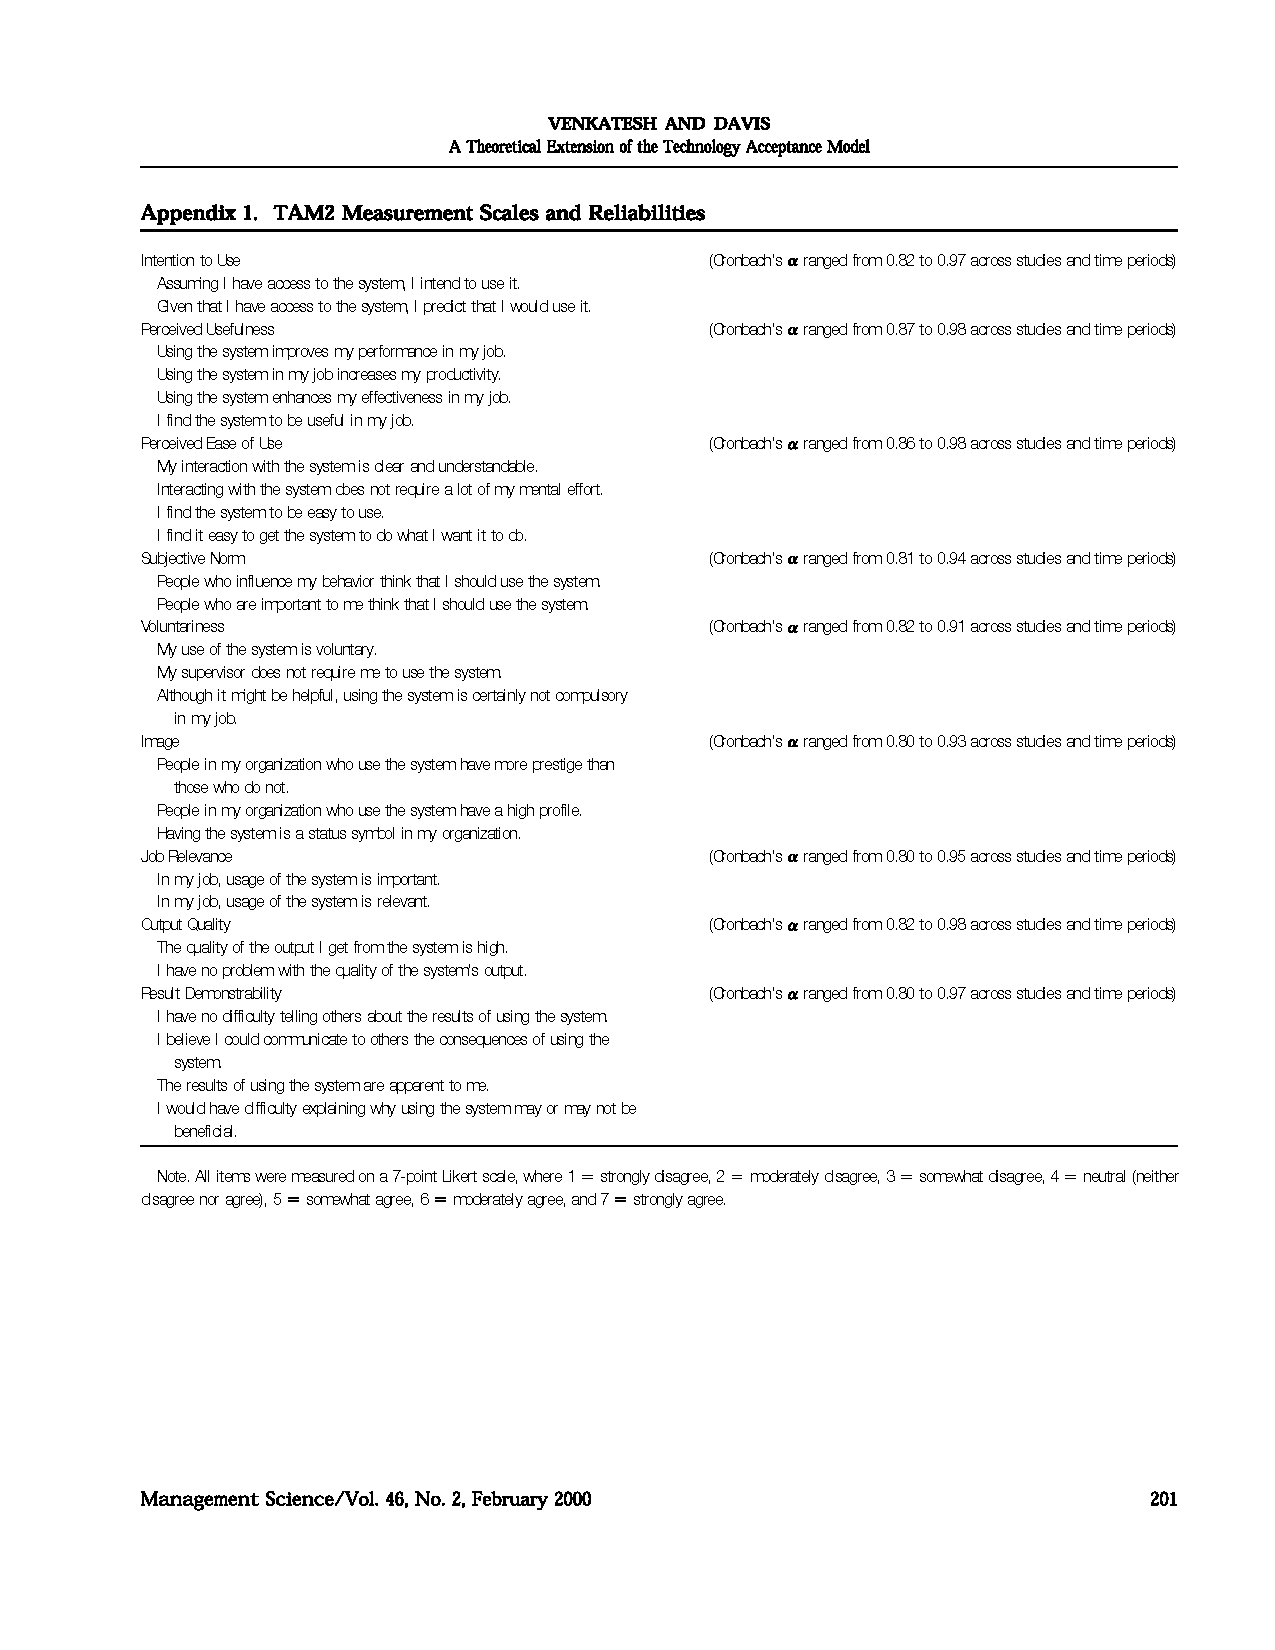
\includegraphics[trim={25mm 60mm 10mm 0mm}]{pdf/TAM2.pdf}

\clearpage
\chapter{Appendix B: Sample Size R Code}
\begin{figure}[h]
    \centering
    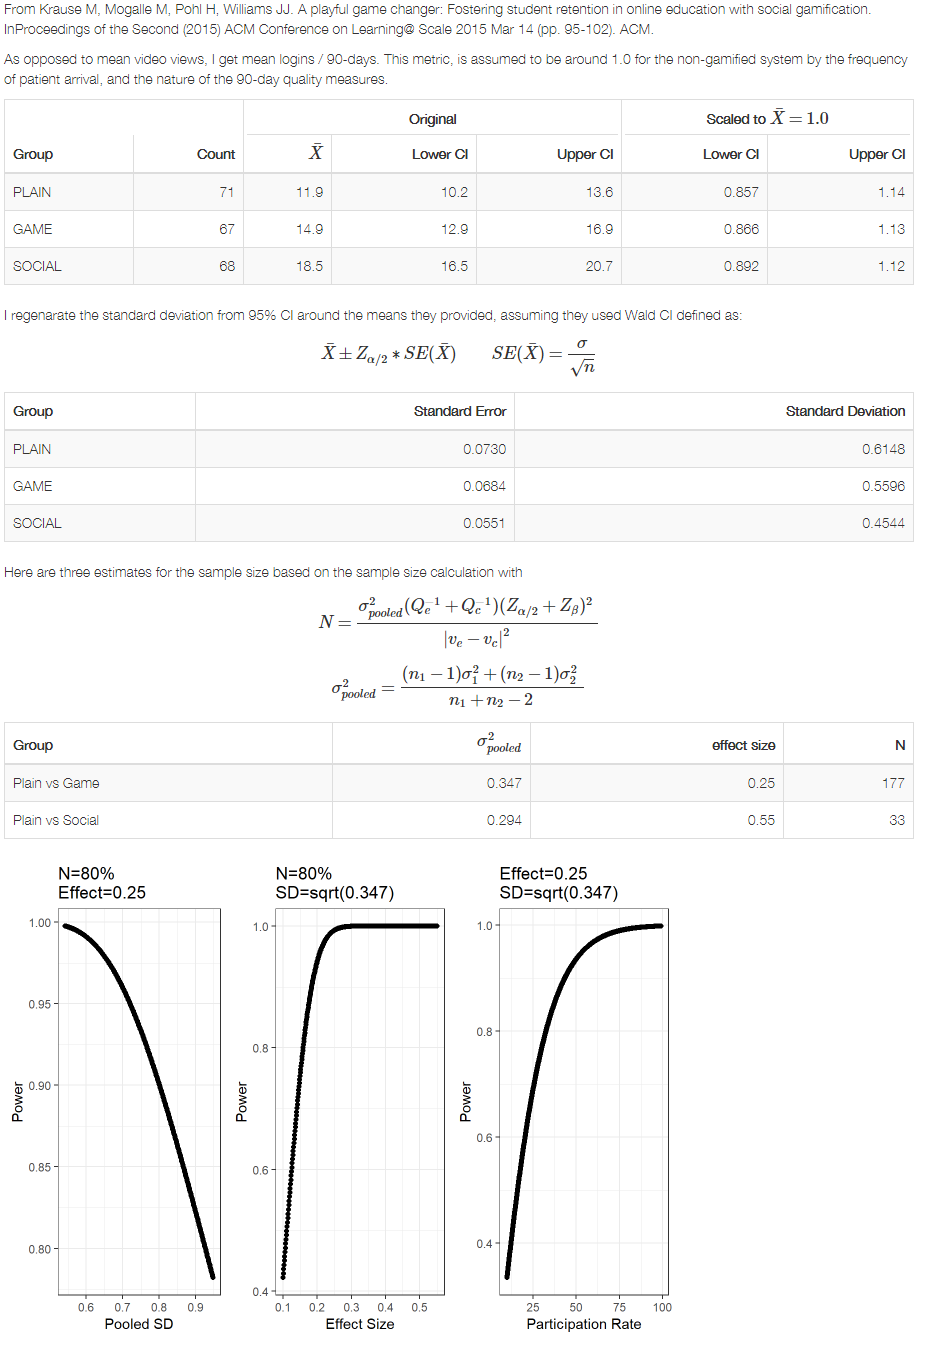
\includegraphics[trim={25mm 10mm 10mm 0mm}, height=0.85\textheight]{img/sample-size.png}
\end{figure}

\end{document}